\PassOptionsToPackage{unicode}{hyperref}
\PassOptionsToPackage{hyphens}{url}

\documentclass[10pt]{article}

\usepackage[margin=0.8in]{geometry}

\usepackage[T1]{fontenc}
\usepackage[utf8]{inputenc}

\usepackage{xcolor}
\usepackage{amsmath,amssymb}
\usepackage{algorithm}
\usepackage{algpseudocode}
\usepackage{graphicx}
\usepackage{tikz}
\usepackage{float}
\usepackage{longtable,booktabs,array,tabularx}
\usepackage{calc}
\usepackage{etoolbox}
\IfFileExists{microtype.sty}{\usepackage{microtype}}{}
\usepackage{hyperref}
\usepackage{bookmark}
\IfFileExists{xurl.sty}{\usepackage{xurl}}{} % safer than unconditional
\urlstyle{same}
\setcounter{secnumdepth}{3}
\setlength{\emergencystretch}{3em}
\setlength{\parskip}{0pt}
\setlength{\parindent}{1em}
\setlength{\textfloatsep}{8pt plus 2pt minus 2pt}
\setlength{\floatsep}{8pt plus 2pt minus 2pt}
\setlength{\intextsep}{8pt plus 2pt minus 2pt}
% --- Fix unicode chars that break pdfLaTeX (arXiv-friendly) ---
\usepackage{newunicodechar}
\newunicodechar{≤}{$\le$}
\newunicodechar{≥}{$\ge$}
\newunicodechar{≈}{$\approx$}
\newunicodechar{±}{$\pm$}
\newunicodechar{Θ}{$\Theta$}
\newunicodechar{Ω}{$\Omega$}
\newunicodechar{ω}{$\omega$}
\newunicodechar{ρ}{$\rho$}
\newunicodechar{Σ}{$\Sigma$}

\makeatletter
\patchcmd\longtable{\par}{\if@noskipsec\mbox{}\fi\par}{}{}
\makeatother

\hypersetup{
  pdftitle={LadderSort: Adaptive Subsequence-Based Sorting Algorithm},
  hidelinks,
  pdfcreator={LaTeX}
}

\title{LadderSort: Adaptive Sorting via Interleaved Nondecreasing Subsequences}

\author{%
  Malik Mir Hamza Nayab\textsuperscript{1}\thanks{Email: \href{mailto:hamza.nayab48@gmail.com}{hamza.nayab48@gmail.com}} \and
  Ghanwa Batool\textsuperscript{2}\thanks{Email: \href{mailto:ghanwa@cuiatd.edu.pk}{ghanwa@cuiatd.edu.pk}}\\[0.5em]
  \textsuperscript{1,2}Comsats University Islamabad, Abbottabad Campus, Pakistan
}

\date{}

\begin{document}
\maketitle

\begin{abstract}
Many data-processing workloads produce sequences that are not globally sorted but are interleavings of locally ordered streams. We present \emph{LadderSort}, an adaptive sorting algorithm for inputs that can be decomposed into interleavings of nondecreasing subsequences. The raw algorithm, which is the main algorithmic contribution, performs a deterministic left-to-right decomposition into ladders followed by an adaptive merge whose cost depends on the measured ladder count \(K\). LadderSort differs from natural run-adaptive methods such as TimSort by adapting to the number of interleaved nondecreasing subsequences \(K\), rather than the number of contiguous runs. We also evaluate Hybrid LadderSort, a practical guardrail that falls back on high-\(K\) inputs to reduce worst-case exposure without replacing the raw \(K\)-adaptive design. The evaluation combines synthetic workloads, a controlled \(K\)-sweep, ablation experiments, hybrid evaluation, memory and comparison-overhead measurements, and one real GH Archive event trace. The real trace contains 55,364 records from 12,783 sources and has measured \(K=368\), indicating nontrivial interleaved-stream structure. Across the experimental suite, LadderSort is strongest on small-\(K\) interleaved workloads and is competitive with TimSort in such regimes, while \texttt{std::sort} remains a strong baseline on unstructured or random inputs. These results support LadderSort as a deterministic, structure-adaptive alternative for workloads where noncontiguous order is present.
\end{abstract}

\noindent\textbf{Keywords:} adaptive sorting; nondecreasing subsequences; multiway merge; loser tree; presortedness; streaming data; performance evaluation

\clearpage

\section{Introduction}

Sorting is a fundamental primitive in computing systems, underpinning database operators, stream-processing pipelines, search indexing, analytics, and online services. Classical comparison-based algorithms provide robust worst-case guarantees, but for an input of length \(N\), their performance is usually characterized by \(\Theta(N\log N)\) even when the input contains latent order. Practical sorting libraries therefore incorporate adaptivity. TimSort, for example, detects contiguous monotone runs and merges them using carefully engineered policies. This form of adaptivity is highly effective when order appears as long adjacent segments, but it is less directly matched to workloads where order is present but noncontiguous.

In many modern systems, data arrives as a fan-in of locally ordered producers. Social feeds combine events from multiple accounts, telemetry systems merge timestamped records from distributed devices, market-data systems aggregate venue-specific streams, and search systems merge partial posting-list segments. In such settings, each producer may emit a locally nondecreasing stream, while the observed global sequence is a bursty interleaving of those streams. The resulting input can contain many short contiguous runs even though it is structurally close to an interleaving of only \(K\) nondecreasing subsequences. We use \(K\) to denote the measured number of ladders produced by the decomposition used in this paper.

This paper introduces \emph{LadderSort}, a deterministic adaptive sorting algorithm for this noncontiguous form of order. LadderSort differs from natural run-adaptive methods such as TimSort by adapting to the number of interleaved nondecreasing subsequences \(K\), rather than the number of contiguous runs. The raw LadderSort algorithm is the main contribution. It performs a single left-to-right decomposition into ladders, assigning each key to the leftmost ladder whose tail is \(\le\) the key while maintaining ladder tails in nonincreasing order. A locality-aware hinted search reduces placement overhead in practice. The resulting ladders are then merged using a strategy selected by \(K\): direct return for \(K=1\), a two-way galloping merge for \(K=2\), and a deterministic loser-tree merge for \(K>2\).

The resulting cost is \(O(N\log K)\) with \(O(N+K)\) auxiliary space. Thus, LadderSort is strongest when \(K\) is small relative to \(N\), and it degrades toward ordinary \(N\log N\) behavior as \(K\) grows. This is a structural claim rather than a universal speed claim: unstructured inputs and highly optimized in-place baselines such as \texttt{std::sort} can remain preferable. The implementation also makes a deliberate determinism trade-off. Equal keys are resolved during multiway merge by a fixed ladder-identifier tie-break, yielding reproducible output under duplicate-heavy inputs but not guaranteeing global stability with respect to original input order across ladders.

We also evaluate \emph{Hybrid LadderSort}, a practical extension that monitors \(K\) during decomposition and falls back when the input enters a high-\(K\) regime. This hybrid is a guardrail rather than a replacement for the raw algorithmic contribution: its purpose is to reduce exposure to unfavorable inputs while preserving the small-\(K\) path when the ladder count remains low.

\noindent\textbf{Contributions.}
\begin{itemize}
\item We present a deterministic online decomposition of an input into nondecreasing ladders, producing a measured structure parameter \(K\).
\item We design a merge strategy that gives \(O(N\log K)\) behavior and strong performance on small-\(K\) interleaved workloads.
\item We introduce a hybrid guardrail that falls back in high-\(K\) regimes while preserving the small-\(K\) behavior of the raw algorithm.
\item We provide a reproducible experimental evaluation covering synthetic workloads, a controlled \(K\)-sweep, ablations, hybrid behavior, memory and comparison overheads, and one real GH Archive event trace.
\end{itemize}

\clearpage

\section{Related Work}\label{related-work}

\subsection{General-Purpose Comparison Sorts}\label{general-purpose-comparison-sorts}

Classical comparison sorts and their hybrids, including introsort, pattern-defeating quicksort, and BlockQuicksort, provide strong worst-case or practical performance but do not parameterize cost by noncontiguous latent order \([1,14,15]\). Smoothsort is adaptive on already sorted input while preserving \(O(n\log n)\) worst-case time \([2]\), but it does not target interleavings of a small number of sorted streams.

\subsection{Run-Adaptive Natural Merges}\label{run-adaptive-natural-merges}

Natural mergesorts exploit contiguous monotone runs. TimSort detects ascending or descending runs, uses galloping, and has worst-case \(O(n\log n)\) behavior with adaptivity to the number of runs \(\rho\) \([3]\). PowerSort, Multiway PowerSort, and AdaptiveShiversSort improve merge scheduling for such run-adaptive settings \([4\text{--}6]\). LadderSort is complementary: it adapts to noncontiguous ladders \(K\), not to contiguous runs \(\rho\).

\subsection{Measures of Presortedness and Adaptive Sorting}\label{measures-of-presortedness}

Adaptive-sorting theory relates running time to disorder measures such as runs, inversions, oscillations, exchanges, and entropy \([7,8]\). Skiena's encroaching lists are especially close in spirit: they build monotone subsequences as a presortedness measure \([9]\). LadderSort uses a simpler tail-guided placement rule and then merges the resulting ladders explicitly.

\subsection{Sequence Decomposition and LIS/LDS Connections}\label{sequence-decomposition}

Classical decomposition results connect monotone subsequence covers with decreasing-subsequence structure; in the offline setting, patience sorting and chain-decomposition views give the relevant background \([10\text{--}12]\). LadderSort uses these ideas only as motivation. It does not compute a minimum chain decomposition offline; it constructs a deterministic online decomposition whose cost is governed by the resulting measured \(K\).

\subsection{Multiway Merging and Tournament/Loser Trees}\label{multiway-merging}

Tournament trees and loser trees are standard tools for \(K\)-way merging, with \(O(K)\) build time and \(O(\log K)\) work per extracted element \([1,13]\). LadderSort uses this classical merge primitive after constructing its ladders.

\section{Materials and Methods}\label{materials-and-methods}

\subsection{Methodology Overview}\label{methodology-overview}

LadderSort has two phases: a single scan that decomposes the input into nondecreasing ladders, followed by a merge chosen from the measured ladder count \(K\).

\begin{figure}[H]
\centering
\resizebox{\linewidth}{!}{%
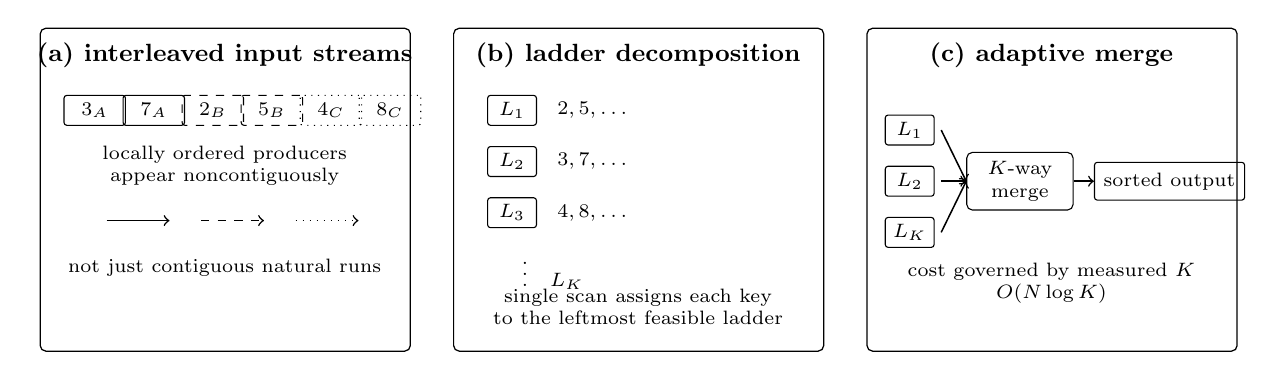
\begin{tikzpicture}[
  panel/.style={draw, rounded corners=2pt, line width=0.45pt,
    minimum width=4.7cm, minimum height=4.1cm, anchor=north west},
  token/.style={draw, rounded corners=1pt, minimum width=0.62cm,
    minimum height=0.38cm, inner sep=1pt, font=\scriptsize},
  stream/.style={draw, rounded corners=1pt, minimum width=0.78cm,
    minimum height=0.38cm, inner sep=1pt, font=\scriptsize},
  arrow/.style={->, line width=0.55pt},
  title/.style={font=\bfseries\small},
  note/.style={font=\scriptsize, align=center},
  every node/.style={font=\small}
]
\node[panel] (a) at (0,0) {};
\node[panel] (b) at (5.25,0) {};
\node[panel] (c) at (10.5,0) {};

\node[title] at (2.35,-0.35) {(a) interleaved input streams};
\node[title] at (7.60,-0.35) {(b) ladder decomposition};
\node[title] at (12.85,-0.35) {(c) adaptive merge};

\node[stream] at (0.70,-1.05) {\(3_A\)};
\node[stream] at (1.45,-1.05) {\(7_A\)};
\node[stream,dashed] at (2.20,-1.05) {\(2_B\)};
\node[stream,dashed] at (2.95,-1.05) {\(5_B\)};
\node[stream,dotted] at (3.70,-1.05) {\(4_C\)};
\node[stream,dotted] at (4.45,-1.05) {\(8_C\)};
\node[note] at (2.35,-1.75) {locally ordered producers\\appear noncontiguously};
\draw[arrow] (0.85,-2.45) -- (1.65,-2.45);
\draw[arrow,dashed] (2.05,-2.45) -- (2.85,-2.45);
\draw[arrow,dotted] (3.25,-2.45) -- (4.05,-2.45);
\node[note] at (2.35,-3.05) {not just contiguous natural runs};

\node[token] at (6.00,-1.05) {\(L_1\)};
\node[anchor=west, font=\scriptsize] at (6.45,-1.05) {\(2,5,\ldots\)};
\node[token] at (6.00,-1.70) {\(L_2\)};
\node[anchor=west, font=\scriptsize] at (6.45,-1.70) {\(3,7,\ldots\)};
\node[token] at (6.00,-2.35) {\(L_3\)};
\node[anchor=west, font=\scriptsize] at (6.45,-2.35) {\(4,8,\ldots\)};
\node[anchor=west, font=\scriptsize] at (6.00,-3.05) {\(\vdots\quad L_K\)};
\node[note] at (7.60,-3.55) {single scan assigns each key\\to the leftmost feasible ladder};

\node[token] at (11.05,-1.30) {\(L_1\)};
\node[token] at (11.05,-1.95) {\(L_2\)};
\node[token] at (11.05,-2.60) {\(L_K\)};
\node[draw, rounded corners=2pt, minimum width=1.35cm, minimum height=0.68cm,
  font=\scriptsize, align=center] (merge) at (12.45,-1.95) {\(K\)-way\\merge};
\node[draw, rounded corners=1pt, minimum width=1.55cm, minimum height=0.48cm,
  font=\scriptsize] (out) at (14.35,-1.95) {sorted output};
\draw[arrow] (11.45,-1.30) -- (merge.west);
\draw[arrow] (11.45,-1.95) -- (merge.west);
\draw[arrow] (11.45,-2.60) -- (merge.west);
\draw[arrow] (merge.east) -- (out.west);
\node[note] at (12.85,-3.25) {cost governed by measured \(K\)\\\(O(N\log K)\)};
\end{tikzpicture}%
}
\caption{LadderSort decomposes noncontiguous ordered streams into ladders and merges them with cost governed by measured \(K\).}
\label{fig:overview}
\end{figure}

\subsection{Two-Phase Description}\label{two-phase}

\paragraph{Phase 1 (decomposition).}
The scan appends each key \(x\) to the leftmost ladder whose tail is \(\le x\); if none exists, it creates a new ladder. The tail array \texttt{tops} is maintained in nonincreasing order and searched with a local hint, galloping, and binary search.

\paragraph{Phase 2 (merge).}
The merge phase returns the ladder directly for \(K=1\), uses a two-way galloping merge for \(K=2\), and uses a loser-tree \(K\)-way merge for \(K>2\). Thus the merge height is controlled by \(K\).


\section{Algorithm (Formal Definition)}
\label{sec:algorithm}

\subsection{\textbf{Problem Setting and Notation}}
Let \(A=\langle a_1,\dots,a_N\rangle\) be keys from a totally ordered domain \((\mathcal{D},\le)\), and let \([m]=\{1,\dots,m\}\). The goal is to output a nondecreasing permutation \(S\) of \(A\).

\paragraph{Deterministic tie handling (implementation).}
Placement uses \(\texttt{tops}[j]\le x\). During merge, equal keys are ordered by ladder id (Definition~5), giving reproducible output under duplicates but not global stability by original input position.


\subsection{\textbf{Ladders and the Parameter $K$}}

\paragraph{Definition 1 (Ladder).}
A \emph{ladder} is a finite nondecreasing sequence \(L=\langle \ell_1,\dots,\ell_m\rangle\):
\[
\ell_1 \le \ell_2 \le \cdots \le \ell_m,
\]


\paragraph{Definition 2 (Tail and tail array).}
For a nonempty ladder \(L\), \(\mathrm{tail}(L)=\ell_m\). Phase~1 maintains ladders \((L_1,\dots,L_K)\) and \(\texttt{tops}[j]=\mathrm{tail}(L_j)\), with invariant
\[
\texttt{tops}[1] \ge \texttt{tops}[2] \ge \cdots \ge \texttt{tops}[K].
\]

\paragraph{Definition 3 (Placement index).}
For key \(x\), define
\[
\pi(x; \texttt{tops}) := \min\{ j \in [K] : \texttt{tops}[j] \le x \},
\]
or \(\pi(x;\texttt{tops})=K+1\) if no feasible ladder exists.

\paragraph{Definition 4 (Formal definition of \(K\)).}
\(K\) is the number of ladders produced by the deterministic Phase~1 placement rule. It is algorithm-induced and is not assumed to be the minimum possible number of nondecreasing subsequences.

\subsection{\textbf{Phase 1: Tail-Guided Decomposition}}

\paragraph{Invariant (Phase 1).}
After processing the prefix $\langle a_1,\dots,a_t\rangle$, the algorithm maintains:
(i) each $L_j$ is a ladder (nondecreasing),
(ii) $\texttt{tops}[j]=\mathrm{tail}(L_j)$, and
(iii) $\texttt{tops}$ is nonincreasing.

\begin{algorithm}[H]
\caption{\textsc{LadderSort}$(A)$ (formal)}
\label{alg:laddersort}
\begin{algorithmic}[1]
\Require $A=\langle a_1,\dots,a_N\rangle$
\Ensure Sorted sequence $S$
\State Initialize an empty list of ladders $(L_1,\dots,L_K)$ with $K\gets 0$
\State Initialize empty array $\texttt{tops}$
\State $\texttt{lastIdx} \gets 1$ \Comment{hint for locality; arbitrary when $K=0$}
\For{$i = 1$ to $N$}
    \State $x \gets a_i$
    \State $j \gets \textsc{HintedLowerBoundNonIncreasing}(\texttt{tops}, x, \texttt{lastIdx})$
    \Comment{$j$ returns $\pi(x;\texttt{tops})$ in Definition~3}
    \If{$j = K+1$}
        \State $K \gets K+1$
        \State $L_K \gets \langle x\rangle$
        \State $\texttt{tops}[K] \gets x$
    \Else
        \State Append $x$ to the end of $L_j$
        \State $\texttt{tops}[j] \gets x$
    \EndIf
    \State $\texttt{lastIdx} \gets j$
\EndFor
\State \Return \textsc{MergeByK}$(L_1,\dots,L_K)$
\end{algorithmic}
\end{algorithm}

\paragraph{Implementation note (search).}
\textsc{HintedLowerBoundNonIncreasing} returns the first \(j\) with \(\texttt{tops}[j]\le x\), using a local probe, exponential gallop, and binary search.

\subsection{\textbf{Phase 2: Merge and Formal Tie-Breaking}}

\paragraph{Definition 5 (Run identifier tie-break).}
Each ladder receives a fixed id \(j\in[K]\). During \(K\)-way merge, heads are compared by
\[
(x,j) \prec (y,\ell) \iff (x<y)\ \lor\ (x=y\ \wedge\ j<\ell).
\]
This deterministic tie-break is not a global stability guarantee across ladders.


\begin{algorithm}[H]
\caption{\textsc{MergeByK}$(L_1,\dots,L_K)$}
\label{alg:mergebyk}
\begin{algorithmic}[1]
\Require Ladders $L_1,\dots,L_K$ (each nondecreasing)
\Ensure Sorted merge $S$
\If{$K=0$} \State \Return $\langle\rangle$ \EndIf
\If{$K=1$} \State \Return $L_1$ \EndIf
\If{$K=2$} \State \Return \textsc{TwoWayMergeWithGalloping}$(L_1,L_2)$ \EndIf
\State \Return \textsc{KWayMergeLoserTree}$(L_1,\dots,L_K)$ \Comment{uses Definition~5}
\end{algorithmic}
\end{algorithm}

\paragraph{Loser-tree merge.}
The loser tree keeps one current head per ladder, outputs the minimum under Definition~5, advances that ladder, and restores the tournament in \(O(\log K)\) time.

\subsection{\textbf{Complexity}}
Phase~1 performs $N$ placements, each costing $O(\log K)$ worst-case, yielding $O(N\log K)$ time.
Phase~2 costs $O(N)$ for $K\in\{1,2\}$ and $O(N\log K)$ for $K>2$ (after $O(K)$ initialization).
Auxiliary space is $O(N+K)$ to store ladders and merge state.

\section{\textbf{Correctness Proof}}
\label{sec:correctness}

\subsection{\textbf{Proof sketch}}
\label{lem:ladder_sorted}
\label{lem:tops_nonincreasing}
\label{lem:merge_sorted}
\label{lem:complexity}
\label{thm:correctness}

Phase~1 appends a key \(x\) only to a ladder whose current tail is \(\le x\);
otherwise it creates a new one-element ladder. Thus each ladder remains
nondecreasing. The same placement rule preserves the nonincreasing order of
\texttt{tops}: replacing the first tail \(\le x\) keeps all earlier tails above
\(x\), while all later tails are already no larger than the replaced tail; a new
ladder is appended only when \(x\) is smaller than every current tail.

After decomposition, Phase~2 merges sorted ladders. The cases \(K=0\) and
\(K=1\) are immediate, \(K=2\) is a standard two-way merge, and \(K>2\) uses a
loser tree to repeatedly output the smallest current ladder head. The
tie-breaker in Definition~5 orders equal keys by ladder id, so output is
deterministic but not globally stable by original position. Since each merge
step consumes exactly one input element and outputs it once, the result is a
sorted permutation of the input.

For complexity, Phase~1 performs \(N\) searches over \texttt{tops}, each costing
\(O(\log K)\) in the worst case. Phase~2 is linear for \(K\le2\), and for
\(K>2\) the loser tree costs \(O(K)\) to build and \(O(\log K)\) per output.
Since \(K\le N\), the total time is \(O(N\log K)\), with \(O(N+K)\) auxiliary
space for ladders and merge state. \(\square\)


\subsection{Implementation Flowchart}
\label{flowchart-of-laddersort}

\begin{figure}[H]
\centering
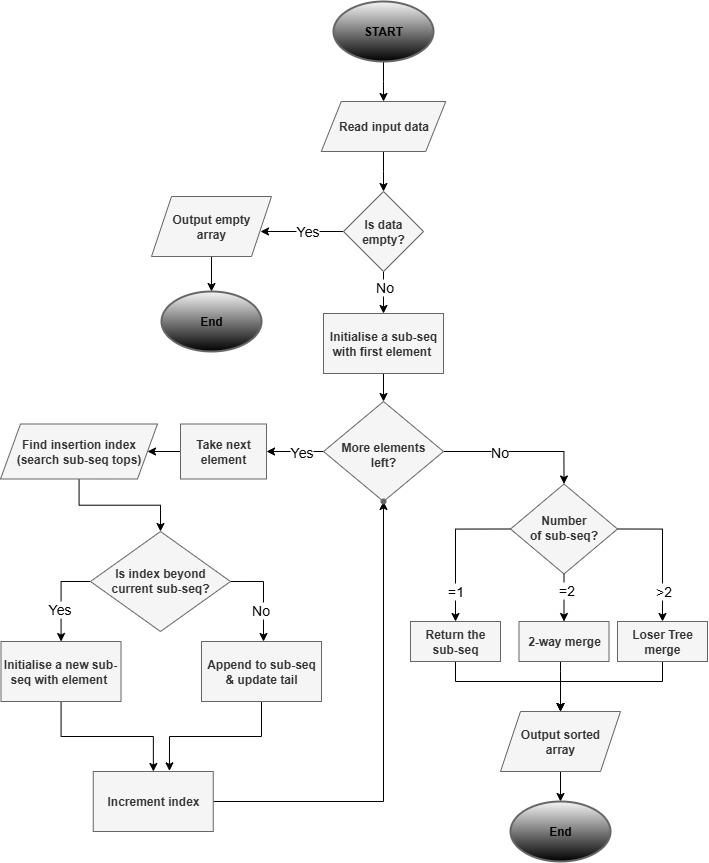
\includegraphics[width=0.48\linewidth]{media/media/image2.jpg}
\caption{Implementation flowchart for LadderSort.}
\label{fig:laddersort-flowchart}
\end{figure}
\section{Experimental Setup}\label{experimental-setup}

All experiments were executed on a 2020 MacBook Air featuring an Apple M1 8-core CPU and 8 GB of unified memory, running macOS 15.6.1. Implementations were compiled using Homebrew GCC 15 with C++20 and the following flags:
\[
\texttt{/opt/homebrew/bin/g++-15 -O3 -march=native -flto -funroll-loops -std=c++20}.
\]
All binaries were single-threaded and used only the compiler’s auto-vectorization (no explicit SIMD or parallelism).

\subsection{Algorithms Under Comparison}\label{algorithms-under-comparison}

\begin{itemize}
\item \textbf{LadderSort (this work):} deterministic two-phase ladder construction followed by adaptive merge (two-way galloping or \(K\)-way loser-tree).
\item \textbf{TimSort:} stable adaptive mergesort (we use \texttt{gfx::timsort}).
\item \textbf{QuickSort:} unstable in-place quicksort with three-way partitioning and median-of-three/ninther pivoting.
\item \textbf{IntroSort:} C++ \texttt{std::sort}.
\item \textbf{StableSort:} C++ \texttt{std::stable\_sort}.
\item \textbf{MergeSort:} reference top-down stable mergesort with a reusable buffer.
\end{itemize}

\subsection{Measured \(K\) and Controlled \(K\)-Sweep Protocol}
\label{k-measurement-protocol}

We measure \(K\) using the same deterministic tail-guided placement rule as Phase~1, but without performing the final merge. For the main workloads, \(K\) is recorded for every dataset, size, and seed, and the resulting measurements are summarized using mean, median, minimum, and maximum values.

For the controlled \(K\)-sweep, we generate randomized exact-\(K\) interleavings at \(N=10^7\). The generator creates exactly the target number of ladders while avoiding repeated descending blocks that would favor run-adaptive baselines. We report median time over 10 timed rounds after one warm-up. The raw data and unfiltered summary are retained; the paper figures use a filtered summary that removes extreme \(\texttt{time\_sec} > 10.0\)s outliers caused by system-level paging or background noise. This filtering removed 6 of 400 rows (1.5\%); all correctness checks passed, and all filtered groups retained at least 8 samples.

\subsection{Overhead Measurement Protocol}
\label{overhead-measurement-protocol}

To evaluate overhead beyond wall-clock time, we measure peak memory and key-comparison counts. Peak memory is measured as maximum resident set size on macOS. The memory experiment uses the random, descending, and social-feed workloads. We run three seeds at \(N=10^7\), and one seed at \(N=10^8\) as a larger stress case.

Comparison counts are measured on smaller inputs because instrumentation changes constant factors. We run \(N=10^5\) and \(N=10^6\) on random, descending, block-cyclic, two-run riffle, and social-feed workloads, using five seeds per configuration. For LadderSort, comparisons are counted inside the hinted placement search, the two-way merge, and the loser-tree merge. For TimSort, \texttt{std::sort}, and \texttt{std::stable\_sort}, we sort wrapped keys using a comparator that increments a counter. Move/write counts are intentionally omitted from this phase to avoid invasive instrumentation; memory and comparison counts are the primary overhead evidence.

\subsection{Real-World Trace Protocol}
\label{real-trace-protocol}

To complement the synthetic workloads, we evaluate one public real-world event trace derived from GH Archive \([16]\). GH Archive records the public GitHub event timeline and provides hourly JSON archives. We use eight hourly archives from 2015-01-01 at 0, 3, 6, 9, 12, 15, 18, and 21 UTC.

Each event provides a timestamp and repository metadata. We use \texttt{created\_at} as the sortable key and \texttt{repo.id} as the source identifier when available, falling back to \texttt{repo.name}. We drop rows missing either field, keep sources with at least two events, sort events within each source by timestamp, and then build a deterministic sticky-burst interleaving of the source streams. This preserves local timestamp order inside each repository stream while avoiding a globally sorted input. The resulting trace contains 55,364 records from 12,783 sources.

This trace is intended to test whether the structural premise of LadderSort appears in a public event stream. GitHub events are generated by many repositories, each of which can be viewed as a local event stream, while the benchmark sequence is an interleaving of those repository-level streams.

\section{\texorpdfstring{\textbf{Results and Discussion}}{Results and Discussion}}\label{results-and-discussion}

The empirical evaluation proceeds in stages. We first establish baseline
runtime behavior across the synthetic workloads, then relate those results to
the measured ladder count \(K\) and to values obtained from a controlled
\(K\)-sensitivity sweep. Next, we ablate the main implementation choices,
evaluate Hybrid LadderSort as a guardrail for high-\(K\) inputs, report memory
and comparison-count overheads, and finally test one public GH Archive event
trace.

The runtime evaluation compares LadderSort with several baseline sorting
algorithms under a range of input distributions. For each workload, we sort
arrays of 1 million, 10 million, and 100 million 32-bit integers. Each
configuration (algorithm, workload, size) is run 10 times; we report mean
wall-clock time and standard deviation. For the controlled \(K\)-sweep, we
report median runtime because a small number of system-level outliers appeared
during long benchmark runs; both unfiltered and filtered summaries are retained
for reproducibility. Unless otherwise stated, all algorithms use the same
toolchain and flags, run single-threaded, and check correctness after every run
with a standard sortedness check.

The algorithms compared are LadderSort (this work), TimSort, QuickSort
(our 3-way partition implementation), IntroSort (C++ \texttt{std::sort}),
StableSort (C++ \texttt{std::stable\_sort}), and a reference MergeSort
(top-down stable mergesort with reusable buffer). The workloads are uniform
random, sorted ascending, sorted descending, band-limited almost-sorted
permutations, block-cyclic interleave, two-run riffle, social-feed fan-in, and
partial index merges.

\subsection{Measured \(K\) and Controlled \(K\)-Sensitivity}
\label{measured-k-and-k-sensitivity}

The measured-\(K\) results make the structural story explicit. Ascending input gives \(K=1\), descending input gives \(K=N\), and the fan-in workloads produce small fixed \(K\). Random inputs produce much larger but still sublinear \(K\), representing the weak-structure regime.

\begin{table}[H]
\centering
\small
\caption{Measured ladder count \(K\) for the main benchmark workloads. Entries are mean ladder counts over 10 runs at each input size \(N\), confirming that the suite spans the intended structural range from \(K=1\) to \(K\approx N\).}
\label{tab:measured-k}
\begin{tabularx}{\linewidth}{@{}lrrrX@{}}
\toprule
Workload & \(N=10^6\) & \(N=10^7\) & \(N=10^8\) & Interpretation \\
\midrule
Ascending & 1.0 & 1.0 & 1.0 & Single ladder \\
Two-run riffle & 2.0 & 2.0 & 2.0 & Two interleaved streams \\
Block-cyclic & 8.0 & 8.0 & 8.0 & Eight producers \\
Band-limited & 14.9 & 15.9 & 16.6 & Bounded local jitter \\
Partial index & 16.0 & 16.0 & 16.0 & Small segment fan-in \\
Social-feed & 24.0 & 24.0 & 24.0 & Multi-source fan-in \\
Random & 1985.8 & 6302.1 & 19955.1 & Weak structure \\
Descending & \(10^6\) & \(10^7\) & \(10^8\) & Worst case \\
\bottomrule
\end{tabularx}
\end{table}

The controlled sweep isolates \(K\) by fixing \(N=10^7\) and varying target \(K\). The randomized exact-\(K\) generator verifies that measured \(K\) equals target \(K\) for every tested value. LadderSort's runtime generally rises with \(K\), which is consistent with the \(O(N\log K)\) analysis.

\begin{figure}[H]
\centering
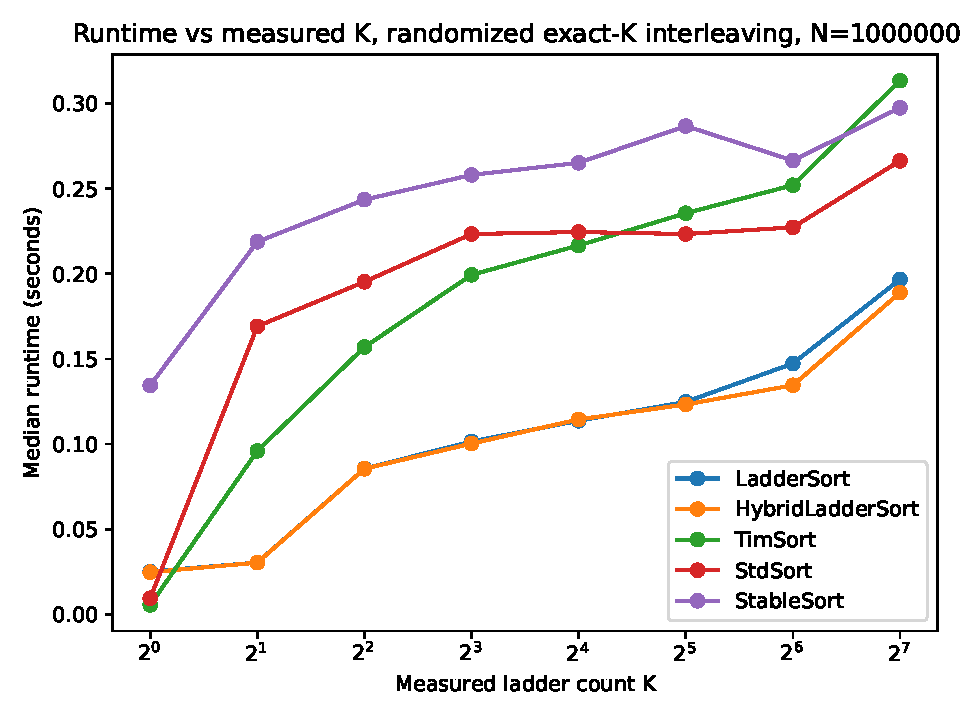
\includegraphics[width=0.82\linewidth]{media/media/k_sweep_runtime_vs_k.pdf}
\caption{Controlled \(K\)-sweep at \(N=10^7\). Median runtime is in seconds and rises with measured \(K\).}
\label{fig:k-sweep-runtime}
\end{figure}

\begin{figure}[H]
\centering
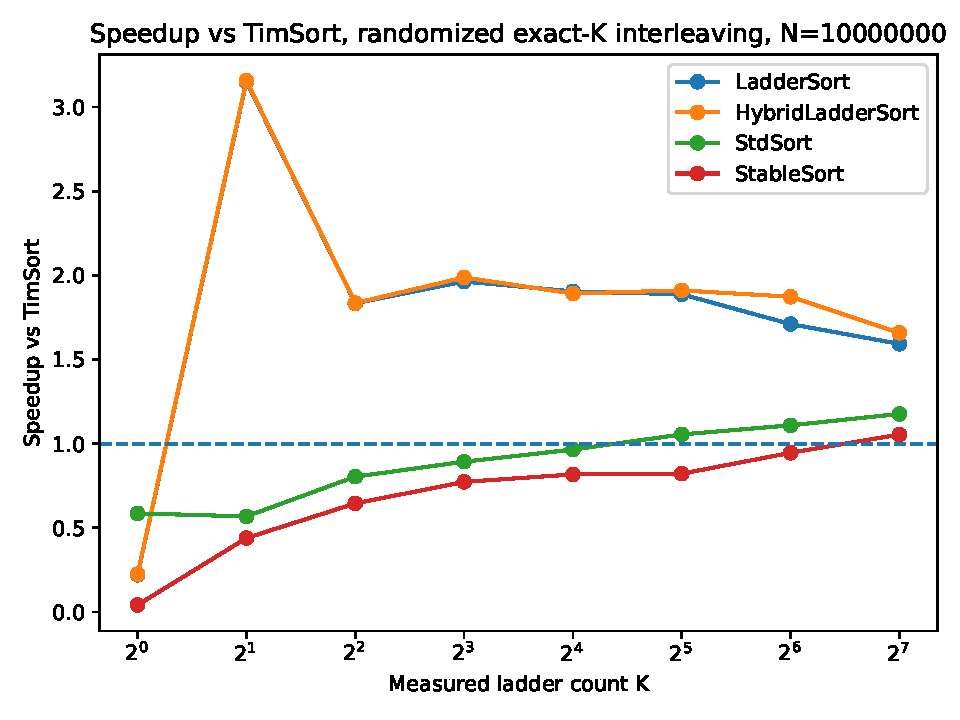
\includegraphics[width=0.82\linewidth]{media/media/k_sweep_speedup_vs_k.pdf}
\caption{Controlled \(K\)-sweep speedup. Values are median runtime ratios relative to TimSort.}
\label{fig:k-sweep-speedup}
\end{figure}

TimSort is fastest at \(K=1\), where the input is a single already sorted run. For small interleaved values of \(K\), LadderSort and Hybrid LadderSort are competitive or faster than TimSort; as \(K\) grows, the advantage narrows. This supports the intended use case: inputs formed by a small number of interleaved ordered streams.

\subsection{Main Runtime Summary}
\label{main-runtime-summary}

The full runtime suite covers eight synthetic workloads at \(10^6\), \(10^7\),
and \(10^8\) elements. To keep the main paper compact,
Table~\ref{tab:runtime-summary-100m} reports the largest-size case. The
complete per-size results remain in the saved result files. The summary keeps
the central pattern: LadderSort is strongest when the input has a small
measured ladder count \(K\), competitive but not dominant on random input, and
weakest on descending input where \(K\approx N\).

\begin{table}[H]
\centering
\scriptsize
\caption{Representative runtime summary at \(N=10^8\). Times are mean seconds over 10 runs.}
\label{tab:runtime-summary-100m}
\begin{tabularx}{\linewidth}{@{}l r r r r X@{}}
\toprule
Workload & Measured \(K\) & LadderSort & TimSort & \texttt{std::sort} & Takeaway \\
\midrule
Uniform random & 19955.1 & 8.352 & 10.021 & 7.286 & \texttt{std::sort} strongest; LadderSort competitive \\
Ascending & 1 & 0.412 & 0.051 & 7.792 & TimSort best on one contiguous run \\
Descending & \(10^8\) & 18.636 & 0.041 & 0.999 & Raw LadderSort worst case; TimSort reverses run \\
Band-limited & 16.6 & 1.928 & 2.520 & 7.975 & Small \(K\) from bounded jitter \\
Block-cyclic & 8 & 0.955 & 1.085 & 4.776 & Eight interleaved producers \\
Two-run riffle & 2 & 1.340 & 1.612 & 4.595 & Two-way merge regime \\
Social-feed & 24 & 1.112 & 1.590 & 9.208 & Tie-heavy small-\(K\) fan-in \\
Partial index & 16 & 1.187 & 1.580 & 3.213 & Repeated-key segment merge \\
\bottomrule
\end{tabularx}
\end{table}

These results explain the broader benchmark behavior. Small-\(K\) interleavings
such as block-cyclic, two-run riffle, social-feed, and partial-index inputs
favor LadderSort because Phase~1 reconstructs the producer-like ladders and
Phase~2 performs a light merge. Random input has weaker structure, so
\texttt{std::sort} remains the best baseline. Ascending input gives \(K=1\),
but TimSort has a smaller constant. Descending input is the raw LadderSort worst
case because it creates one ladder per element; this motivates the hybrid
guardrail evaluated later.

\subsection{Ablation Study}
\label{ablation-study}

The ablation study isolates the main engineering choices inside LadderSort.
We evaluate five variants: LadderFull, NoHint, NoGallop, HeapMerge, and
StableMode. Table~\ref{tab:phase4-ablation} reports median relative time,
normalized to LadderFull for the same workload and size. The social-feed
workload represents the \(K>2\) fan-in regime (\(K=24\)), while two-run
riffle isolates the \(K=2\) merge path.

\begin{table}[H]
\centering
\small
\caption{Phase 4 ablation results. Entries are median relative runtimes normalized to LadderFull \(=1.00\).}
\label{tab:phase4-ablation}
\begin{tabularx}{\linewidth}{@{}l X rrr rrr@{}}
\toprule
& & \multicolumn{3}{c}{Social-feed (\(K=24\))} & \multicolumn{3}{c}{Two-run riffle (\(K=2\))} \\
\cmidrule(lr){3-5}\cmidrule(lr){6-8}
Variant & Purpose & \(10^6\) & \(10^7\) & \(10^8\) & \(10^6\) & \(10^7\) & \(10^8\) \\
\midrule
LadderFull & Full implementation & 1.00 & 1.00 & 1.00 & 1.00 & 1.00 & 1.00 \\
NoHint & Disable hinted placement & 1.71 & 1.75 & 1.28 & 0.86 & 0.84 & 0.68 \\
NoGallop & Disable galloping merge & 0.97 & 0.99 & 0.72 & 1.07 & 1.06 & 0.79 \\
HeapMerge & Replace loser tree with heap & 1.94 & 2.05 & 1.51 & 1.02 & 1.00 & 0.82 \\
StableMode & Preserve global stability & 1.03 & 1.07 & 1.26 & 1.05 & 1.07 & 1.43 \\
\bottomrule
\end{tabularx}
\end{table}

The social-feed ablation demonstrates the significance of both locality-aware
placement search and loser-tree merge, especially in the \(K>2\) fan-in regime.
NoHint hurts performance by \(1.28\times\)--\(1.75\times\) in median time,
while HeapMerge increases median time by \(1.51\times\)--\(2.05\times\). We see
StableMode's overhead most clearly at \(10^8\), where it runs at
\(1.26\times\) the runtime of LadderFull.

Performance results for the \(K=2\) two-run riffle ablation are less clear-cut.
NoGallop is slower at \(10^6\) and \(10^7\), but faster at \(10^8\). NoHint is
also faster on this workload, suggesting the hinted-search cost is not
justified when the decomposition is fixed at two ladders. We therefore consider
NoGallop and NoHint to be workload-sensitive performance optimizations rather
than unequivocally dominant techniques.

\subsection{Hybrid LadderSort}
\label{hybrid-laddersort}

Hybrid LadderSort is a practical safeguard rather than the main algorithmic
contribution. The raw algorithm exposes the structural \(O(N\log K)\) behavior
directly. The hybrid variant monitors the ladder count during decomposition and
falls back when \(K\) exceeds the threshold, aiming to avoid the descending and
random-input worst cases while preserving the small-\(K\) path.

\begin{table}[H]
\centering
\scriptsize
\caption{Hybrid LadderSort evaluation. Speedups are median runtime ratios; fallback rate is the fraction of fallback runs.}
\label{tab:phase4-hybrid}
\begin{tabularx}{\linewidth}{@{}l r r r r X@{}}
\toprule
Dataset & \(N\) & Fallback rate & Hybrid vs Raw & Hybrid vs TimSort & Interpretation \\
\midrule
Descending & \(10^6\) & 1.00 & 5.71 & 0.07 & Avoids raw worst case; TimSort best case \\
Descending & \(10^7\) & 1.00 & 6.36 & 0.07 & Avoids raw worst case; TimSort best case \\
Descending & \(10^8\) & 1.00 & 4.14 & 0.03 & Avoids raw worst case; TimSort best case \\
Random & \(10^6\) & 1.00 & 1.62 & 2.51 & Fallback improves over raw \\
Random & \(10^7\) & 1.00 & 1.67 & 2.66 & Fallback improves over raw \\
Random & \(10^8\) & 1.00 & 1.75 & 2.77 & Fallback improves over raw \\
Block-cyclic & \(10^6\) & 0.00 & 0.90 & 1.81 & Preserves small-\(K\) path \\
Block-cyclic & \(10^7\) & 0.00 & 1.03 & 1.75 & Preserves small-\(K\) path \\
Block-cyclic & \(10^8\) & 0.00 & 1.12 & 1.66 & Preserves small-\(K\) path \\
\bottomrule
\end{tabularx}
\end{table}

Fallback behavior is as desired. On descending and random inputs, Hybrid
LadderSort falls back every time, reducing the cost paid by raw LadderSort on
these unfavorable inputs. On block-cyclic inputs, where \(K=8\), the fallback
rate is \(0.00\). This means the hybrid preserves the small-\(K\) LadderSort
path and remains faster than TimSort. Hybrid LadderSort should be considered a
practical guardrail: it guards against high-\(K\) regimes without altering the
fundamental contribution of the raw algorithm, namely \(K\)-adaptive
decomposition and merge.

\subsection{Memory and Comparison Overheads}
\label{memory-and-comparison-overheads}

We also measure peak resident memory and key-comparison counts. Table~\ref{tab:phase5-memory} reports the \(N=10^8\) one-seed memory stress case; the result pack retains the \(N=10^7\) three-seed runs.

\begin{table}[H]
\centering
\scriptsize
\caption{Peak resident set size at \(N=10^8\), reported in GiB. Hybrid reduces high-\(K\) descending memory use while matching Raw LadderSort on small-\(K\) social-feed input.}
\label{tab:phase5-memory}
\begin{tabular}{@{}lrrrrr@{}}
\toprule
Dataset & Raw & Hybrid & TimSort & \texttt{sort} & \texttt{stable} \\
\midrule
Descending & 3.73 & 1.12 & 1.62 & 1.62 & 1.62 \\
Random & 1.06 & 1.26 & 1.12 & 0.75 & 0.90 \\
Social-feed & 1.82 & 1.82 & 0.78 & 0.75 & 1.12 \\
\bottomrule
\end{tabular}
\end{table}

Raw LadderSort caches ladders and merge state. This cache is costly when \(K=N\): descending input peaks at 3.73~GiB. Hybrid falls back here, cutting this peak down to 1.12~GiB. On social-feed input, \(K\) is low (\(24\)), so Hybrid keeps the raw path and has the same footprint.

Table~\ref{tab:phase5-comparisons} shows median key comparisons per element at \(N=10^6\) over five seeds.

\begin{table}[H]
\centering
\scriptsize
\caption{Median key comparisons per element at \(N=10^6\). Small-\(K\) interleavings require far fewer comparisons for LadderSort than general-purpose baselines.}
\label{tab:phase5-comparisons}
\begin{tabular}{@{}lrrrrrr@{}}
\toprule
Dataset & \(K\) & Raw & Hybrid & TimSort & \texttt{sort} & \texttt{stable} \\
\midrule
Two-run riffle & 2 & 2.00 & 2.00 & 4.93 & 20.89 & 18.96 \\
Block-cyclic & 8 & 4.03 & 4.03 & 6.07 & 23.64 & 25.59 \\
Social-feed & 24 & 3.83 & 3.83 & 6.16 & 17.01 & 18.95 \\
Random & 1985 & 21.24 & 27.19 & 18.63 & 22.26 & 29.90 \\
Descending & \(10^6\) & 22.95 & 3.00 & 1.00 & 3.00 & 37.02 \\
\bottomrule
\end{tabular}
\end{table}

The comparison counts match the structural view. Small-\(K\) interleavings need only about 2--4 comparisons per element for LadderSort. Random input is comparable to general-purpose sorting, and descending input exposes the raw high-\(K\) case; Hybrid reduces that cost by falling back.

\subsection{Real-World GitHub Event Trace}
\label{real-world-github-event-trace}

The synthetic suite controls \(K\), but a public trace gives a credibility check. The GH Archive trace contains 55,364 records from 12,783 repository sources. Raw LadderSort measures \(K=368\), giving \(K/N\approx 0.00665\).

\begin{table}[H]
\centering
\scriptsize
\caption{Real-world GH Archive event-trace benchmark. The trace contains 55,364 records from 12,783 repository sources; times are median seconds over 10 rounds, and speedup is relative to TimSort.}
\label{tab:phase6-real-trace}
\begin{tabular}{@{}lrrrr@{}}
\toprule
Algorithm & Median time (s) & Measured \(K\) & Fallback & Speedup \\
\midrule
Raw LadderSort & 0.002026 & 368 & 0.00 & 1.45 \\
Hybrid LadderSort & 0.001600 & 237 & 1.00 & 1.84 \\
TimSort & 0.002939 & 368 & 0.00 & 1.00 \\
\texttt{std::sort} & 0.001001 & 368 & 0.00 & 2.94 \\
\texttt{std::stable\_sort} & 0.000688 & 368 & 0.00 & 4.27 \\
\bottomrule
\end{tabular}
\end{table}

This table divorces structure from raw speed. Note that Raw LadderSort's
\(K=368\); the trace is nowhere close to random-like under the ladder
decomposition. Raw LadderSort is faster than TimSort, and Hybrid is faster still
because it aggressively picks the conservative fallback path. \texttt{std::sort}
and \texttt{std::stable\_sort} remain faster at this small input size, however.
So the real-trace result is a low-\(K\) structure claim and TimSort-level
competitiveness, not universality.

\subsection{\texorpdfstring{\textbf{Asymptotic Behavior and Structural Interpretation}}{Asymptotic Behavior and Structural Interpretation}}\label{asymptotic-behavior-and-structural-interpretation}

LadderSort's cost follows from the measured ladder count \(K\). Phase~1 performs a hinted search over \texttt{tops}; Phase~2 returns one ladder, performs a two-way merge, or uses a loser tree. Combining the two phases gives
\[
T(N,K)=O(N\log K + K),
\]
which is linear for \(K=1\) and \(\Theta(N\log K)\) for larger \(K\). Table~\ref{tab:parametric-bounds} summarizes the bounds.

{\scriptsize
\begin{longtable}{@{}p{0.14\linewidth}p{0.22\linewidth}p{0.18\linewidth}p{0.42\linewidth}@{}}
\caption{Parametric bounds in terms of input size \(N\) and measured ladder count \(K\).}
\label{tab:parametric-bounds}\\
\toprule
Notation & Time bound & Valid when & Interpretation \\
\midrule
\endfirsthead

\toprule
Notation & Time bound & Valid when & Interpretation \\
\midrule
\endhead

\bottomrule
\endfoot

\bottomrule
\endlastfoot

Big-O & \(O(N\log K + K)\) & All \(K\ge 1\) & Placement + loser-tree merge; \(+K\) is tree build. \\
Big-Theta & \(\Theta(N)\) & \(K=1\) & Single run; scan and return. \\
 & \(\Theta(N\log K)\) & \(K\ge 2\) & Tight bound when merging \(K\) runs. \\
Big-Omega & \(\Omega(N)\) & All \(K\) & Must at least read/output \(N\) items. \\
Little-o & \(o(N\log N)\) & \(K=N^{o(1)}\) (e.g., \(K=O((\log N)^c)\)) & Strictly sub-\(N\log N\) when \(K\) grows sub-polynomially. \\
Little-omega & \(\omega(N)\) & \(K\to\infty\) & Superlinear whenever \(K\) diverges. \\
Space & \(O(N+K)\) &  & Linear buffer for runs/output + \(O(K)\) metadata. \\
\end{longtable}
}

Representative workloads fit this parameterization directly. Ascending input has \(K=1\). Block-cyclic, two-run riffle, social-feed, and partial-index merges have small fixed \(K\). Random inputs have sublinear measured \(K\), but optimized \texttt{std::sort} remains strong. Descending input gives \(K=N\), exposing the raw worst case and motivating the hybrid fallback.

\section{\texorpdfstring{\textbf{Limitations and Threats to Validity}}{Limitations and Threats to Validity}}\label{limitations-and-threats-to-validity}


LadderSort's runtime relies on the empirically determined ladder count \(K\).
LadderSort is expected to perform best for small \(K\) values. As \(K\) trends
towards \(N\), LadderSort's runtime trends towards \(O(N\log N)\), its
worst-case runtime. This occurs for descending input, which has exactly one
element per ladder (\(K=N\)). In this worst case, LadderSort has higher
constants than optimized in-place sorting algorithms. Furthermore, LadderSort
is not in-place. It uses \(O(N+K)\) space to store ladders and merge state, so
its memory consumption is higher than optimized in-place baselines.

Our implemented workloads cover a spectrum of structures, but they are
synthetic and not extracted from natural data. Natural data could have
different distributions of interleaved local order that would affect \(K\). For
instance, different fan-in patterns, burst lengths, duplicate rates, or key
domains/types could affect \(K\). Including a real public trace from GH Archive
helps, but it is only one trace. The evaluation should not be read as saying
that all event streams are low-\(K\), but rather that some real event streams
have interleaved local order.

Implementation and platform will also influence these numbers. We implement
one version of TimSort, using one header-only library. \texttt{std::sort} and
\texttt{std::stable\_sort} rely on the standard library implementation,
allocator, and target machine. Finally, our runs use one ARM laptop, fixed
seeds, and a documented compiler command line. Measurements may change across
different platforms. Hybrid LadderSort reduces high-\(K\) exposure, but its
threshold is a policy choice. More traces, additional key types, stable and
lower-memory variants, and threshold tuning across platforms are natural next
steps.

\section{\texorpdfstring{\textbf{Conclusions and Future Work}}{Conclusions and Future Work}}\label{conclusions-and-future-work}
Ladder sort is a deterministic adaptive sorting algorithm optimal for inputs that are interleaved incrementing subsequences. LadderSort does not adapt to the number of contiguous runs, but rather to the number of interleaved nondecreasing subsequences \(K\). The primary contribution is the raw algorithm, which constructs ladders and merges them in \(O(N\log K)\) time using \(O(N+K)\) auxiliary space.

The experiments confirm the intended use case. LadderSort works best on small-\(K\) interleavings, yet remains competitive on random inputs, and shows its worst case on descending inputs. The ablation, memory, comparison-count, and GH Archive experiments clarify both the engineering costs and the optimal structure for the method. Hybrid LadderSort is optimal for high-\(K\) inputs, but is not a replacement for the raw \(K\)-adaptive algorithm.

In future we will broaden the real-trace evauluation, develop stable and lower memory variant. We will focus on tuning the fallback thresholds, and we will also explore parallel and external-memory variants, which are natural directions because the ladder representation already separates the input into sorted streams.

\section{References}\label{references}

{[}1{]} Knuth, D.E. \emph{The Art of Computer Programming; Volume 3: Sorting and Searching}; 2nd ed.; Addison-Wesley: Reading, MA, USA, 1998.

{[}2{]} Dijkstra, E.W. Smoothsort, an alternative for sorting in situ. EWD 796, 1981.

{[}3{]} Auger, N.; Jugé, V.; Nicaud, C.; Pivoteau, C. On the Worst-Case Complexity of TimSort. In \emph{Proceedings of ESA 2018}; LIPIcs, Volume 112; pp. 4:1--4:13.

{[}4{]} Munro, J.I.; Wild, S. Nearly-Optimal Mergesorts: Fast, Practical Sorting Methods That Excel on Partially Ordered Data. In \emph{Proceedings of ESA 2018}; extended manuscript.

{[}5{]} Cawley Gelling, W.; Nebel, M.E.; Smith, B.; Wild, S. Multiway PowerSort. arXiv 2023, arXiv:2209.06909.

{[}6{]} Jugé, V. Adaptive Shivers Sort: An Alternative Sorting Algorithm. arXiv 2018, arXiv:1809.08411; see also SIAM publication (2020).

{[}7{]} Mannila, H. Measures of Presortedness and Optimal Sorting Algorithms. \emph{IEEE Trans. Comput.} 1985, C-34, 318--325.

{[}8{]} Estivill-Castro, V.; Wood, D. A Survey of Adaptive Sorting Algorithms. \emph{ACM Comput. Surv.} 1992, 24, 441--476.

{[}9{]} Skiena, S.S. Encroaching Lists as a Measure of Presortedness. \emph{BIT Numer. Math.} 1988, 28, 775--784.

{[}10{]} Fredman, M.L. On Computing the Length of Longest Increasing Subsequences. \emph{Discrete Math.} 1975, 11, 29--35.

{[}11{]} Dilworth, R.P. A Decomposition Theorem for Partially Ordered Sets. \emph{Ann. Math.} 1950, 51, 161--166.

{[}12{]} Aldous, D.; Diaconis, P. Longest Increasing Subsequences: From Patience Sorting to the Baik--Deift--Johansson Theorem. \emph{Bull. Am. Math. Soc.} 1999, 36, 413--432.

{[}13{]} Polyntsov, M.; Grigorev, V.; Smirnov, K.; Chernishev, G. Implementing the Comparison-Based External Sort. arXiv 2022, arXiv:2207.12713.

{[}14{]} Edelkamp, S.; Weiß, A. BlockQuicksort: Avoiding Branch Mispredictions in Quicksort. In \emph{Proceedings of ESA 2016}; LIPIcs, Volume 57; pp. 38:1--38:16.

{[}15{]} Peters, O.R.L. Pattern-Defeating Quicksort. arXiv 2021, arXiv:2106.05123.

{[}16{]} GH Archive. Public GitHub Timeline Archive. Available online: \url{https://www.gharchive.org/} (accessed on 7 May 2026).

\end{document}
